\chapter{Esercizi}
\section{Es1}
\subsection{Specifica}
Un gruppo di amici ha inventato un semplice gioco di carte che ha le seguenti regole:
\begin{enumerate}
    \item ogni giocatore riceve N carte di valore crescente da 1 a N;
    \item ogni giocatore gioca una carta consegnandola ad un Arbitro senza vedere quella dell'avversario;
    \item il giocatore che ha giocato la carta più alta ha realizzato una “presa”; se le carte hanno pari valore nessuno prende;
    \item 4. l'Arbitro comunica l'esito della giocata ai giocatori;
    \item 5. si ripete dal punto 2 fino ad esaurimento delle carte;
    \item 6. vince chi ha realizzato più “prese”; se le “prese” sono pari non vince nessuno;
    \item 7. il gioco termina con la dichiarazione “hoVinto” o “nonHoVinto” da parte dei giocatori.
\end{enumerate}
Si chiede di implementare questa specifica in Java utilizzando Thread e monitor.
\\NOTA: per semplicità considerare N=10 e 3 giocatori. Si trascurino i dettagli non precisati nel testo (per esempio non conta l'ordine con cui vengono giocate le carte (punto 2) ...).

\subsection{Analisi}
Ogni giocatore può essere modellato usando un thread.
\begin{itemize}
    \item Un giocatore gioca una carta, aspetta un certo tempo e prova a giocare ancora.
    \item Per poter giocare ancora è necessario che la mano sia finita.
    \item Il thread finisce quando tutte le carte del giocatore sono state giocate e il giocatore ha saputo che se ha vinto o ha perso.
\end{itemize}
L'arbitro è la risorsa condivisa.
\begin{itemize}
    \item Deve implementare un metodo per giocare una carta.
    \item Metodo per annunciare il vincitore.
    \item Deve conoscere il turno attuale.
    \item Deve ricordare lo stato di ogni turno precedente (quali carte sono state giocate e chi ha vinto ogni turno).
\end{itemize}
Il gioco è diviso in turni.
\begin{itemize}
    \item Un giocatore deve aspettare che tutti gli altri abbiano finito per giocare ancora (condizione di accesso alla risorsa).
    \item Il turno è un punto di sincronizzazione. Quando scatta un nuovo turno eventuali giocatori in attesa possono giocare la loro carta.
    \item Un giocatore chiede se ha vinto quando ha giocato tutte le carte, deve essere finito l'ultimo turno.
\end{itemize}

\subsubsection{Class Diagram}
Diagramma delle classi di alto livello con l'obiettivo di identificare chiaramente gli attori coinvolti e le azioni principali. Modellato in UML.
\\Le azioni identificate possono anche non essere implementate sotto forma di metodi di classe.
\begin{center}
    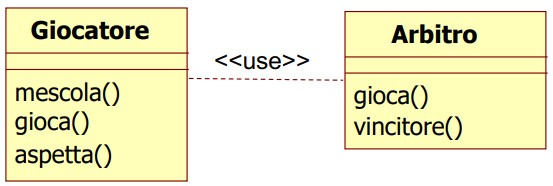
\includegraphics[width=0.5\textwidth]{img/es1_cd1.jpg}
\end{center}

\subsubsection{Giocatore}
Ogni giocatore ha un nome (id numerico) ed N carte (da il cui valore va da 1 a N, semplifichiamo).
\\Il giocatore mescola le carte (--> \textit{shuffle} di numeri interi).
\\Ci sono tanti turni quante carte, quindi ciclicamente succede che:
\begin{itemize}
    \item Il giocatore gioca una carta.
    \item Il giocatore aspetta un certo tempo random e prova a giocare di nuovo.
    \item Se il turno non è finito, il giocatore aspetta (va messo in wait).
\end{itemize}
Quando il giocatore ha finito le carte, questo chiede all'arbitro il nome del vincitore.
\begin{itemize}
    \item Se l'arbitro restituisce il suo id scrive «Sono io il vincitore».
    \item Se l'arbitro restituisce l'id di un altro giocatore scrive «Non ho vinto».
\end{itemize}
Dopo aver stampato a schermo il risultato della partita il thread del giocatore termina.

\subsubsection{Arbitro}
Metodo \verb#gioca(id_giocatore, carta)#
\\Deve essere sincronizzato, solo un giocatore per volta può dare la sua carta
\\Se un giocatore ha già giocato e prova a giocare di nuovo deve essere messo in attesa che
il turno finisca
\\Quando un turno finisce (tutti i giocatori hanno giocato) i giocatori in attesa potranno
essere risvegliati
\\Metodo vincitore()
\\Restituisce l'id del giocatore vincitore
\\Se è sincronizzato possiamo usare wait() per evitare che un giocatore chieda l'esito della
partita prima che questa termini.

\subsection{Implementazione}
\subsubsection{Classe Giocatore:}
\verbatiminput{chaptersLezioni/Giocatore.java}
\subsubsection{Classe Arbitro:}
\verbatiminput{chaptersLezioni/Arbitro.java}
\subsubsection{Classe Main:}
\verbatiminput{chaptersLezioni/Main.java}
